\cotefile{53}
\scanpage{29}
% @ 1–4
d'un monoide affine $G$, cel signifie aussi qu'il existe une opération de $G$ sur $M'$ \deleted{qui} telle que $M\mathrel{\tikz[baseline=-.3ex,x=1em,y=1em]{\draw[line width=.45pt] (0,0)--(1,.05)--(1,-.10);}}M'$ soit comp. avec \unsure{son|ses} op., et il est clair \tikz[baseline=(s.base)]{\node[inner sep=1pt](s){(comme};\node[anchor=south east,inner sep=1pt] at ([xshift=-2pt,yshift=7pt]s.north west){\inserted{\unsure{directemt}}};\draw ([xshift=-10pt,yshift=-1pt]s.south west) to[out=70,in=190] ([xshift=-2pt,yshift=8pt]s.north west) to[out=10,in=250] ([xshift=13pt,yshift=15pt]s.north west);} $W(M)\mathrel{\tikz[baseline=-.3ex,x=1em,y=1em]{\draw[line width=.45pt] (0,0)--(1,.05)--(1,-.10);}}W(M')$ épi) que cette opération sera unique.

% @ 5–6
Si on a un. mono
\[
M''\overset{i}{\hookrightarrow}M
\]
% @ 7–9
alors il ne sera pas vrai en général que $V(M)\mathrel{\tikz[baseline=-.3ex,x=1em,y=1em]{\draw[line width=.45pt] (0,0)--(1,0) (1,-.12)--(1,.12);}}V(M'')$ soit surjectif, ni que $W(M'')\mathrel{\tikz[baseline=-.3ex,x=1em,y=1em]{\draw[line width=.45pt] (0,0)--(1,.05)--(1,-.10);}}W(M)$ soit injectif, donc \unsure{faute de|\deleted{faute de}} cette condition on a du mal à parler d'opération induite.
% @ 10–12
\deleted{\unsure{Crt il est|Cert il est}} On dira qu'il \uline{existe} une op. induite si on peut faire opérer $G$ sur $M''$ de telle façon que $M''\mathrel{\tikz[baseline=-.3ex,x=1em,y=1em]{\draw[line width=.45pt] (0,0)--(1,.05)--(1,-.10);}}M$ soit comp. aux opérations.
% @ 13–15
Mais il n'est plus clair que l'op ``induite'' soit unique ! En termes d'alg. comm., la question est de trouver un $\Delta_{M''}:M''\mathrel{\tikz[baseline=-.3ex,x=1em,y=1em]{\draw[line width=.45pt] (0,0)--(1,.05)--(1,-.10);}}M''\otimes A$ rendant commutatif
% @ 16–18 diagram
\margin{\begin{tikzpicture}[x=1mm,y=1mm]\fill (0,0) ellipse (.4mm and .2mm);\end{tikzpicture}}
\diagram{\begin{tikzcd}[ampersand replacement=\&,row sep=large,column sep=large]
 M'' \arrow[r,dash,"{u_{M''}\,?}",to path={.. controls +(right:4mm) and +(left:4mm) .. (\tikztotarget) \tikztonodes -- ++(-.3pt,-1.4pt)}] \& M''\otimes A \arrow[d,dash,"{i\otimes{\mathrm{id}}_A}",to path={-- (\tikztotarget) \tikztonodes -- ++(.7pt,-1.2pt)}] \\
 M \arrow[u,dash,"i"',to path={-- (\tikztotarget) \tikztonodes .. controls +(up:2pt) and +(up:1pt) .. ++(2.5pt,.2pt)}] \arrow[r,dash,"{u_M}",to path={-- (\tikztotarget) \tikztonodes -- ++(0pt,1.1pt)}] \& M\otimes A
\end{tikzcd}}

% @ 19–20
On peut dire que c'est uniquement déterminé pourvu que $i\otimes{\mathrm{id}}_A=i_A$ soit un mono,
% @ 20 interlinear
\figure{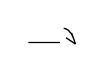
\begin{tikzpicture}[x=1mm,y=1mm]\draw[line width=.45pt] (0,0)--(4,0) (4.5,1.8) to[out=-10,in=110] (6,-.2) (6,-.2)--(5.5,1.2) (6,-.2)--(4.8,.6);\end{tikzpicture}}
\inserted{et si [$\unsure{i|j}\otimes{\mathrm{id}}_{A\otimes A}$ l'est aussi, alors la \unsure{condi.|condt.} \tikz[baseline=(s.base)]{\node[inner sep=1pt](s){\(u_M(M'')\subset\mathrm{Im}\,M''_{\otimes A}\)};\draw[->] ([xshift=-7pt,yshift=10pt]s.north west)--([xshift=-6pt,yshift=-3pt]s.north west)--([xshift=-2pt,yshift=9pt]s.north west);} est néc. et \uline{suffisante} pour la \deleted{\unsure{stabilité}} stabilité ; alors $M'$ est \unsure{stble|stbl} sss $M''$ l'est.}
% @ 21
\deleted{\unsure{batise|banise} \unsure{ces remarques}}. Les conditions envisagées sont ok dans les cas suivants :

% @ 22
a) $A$ est plat$/k$ (p.~ex. $k$ un corps)

% @ 22–24 right margin
\margin{\deleted{Alors les \unsure{c.s.} de \unsure{la} \unsure{q°} \unsure{s'appl.} \unsure{montrent} $u_M(M'')\subset\mathrm{Im}\,M''_{\otimes A}$.} 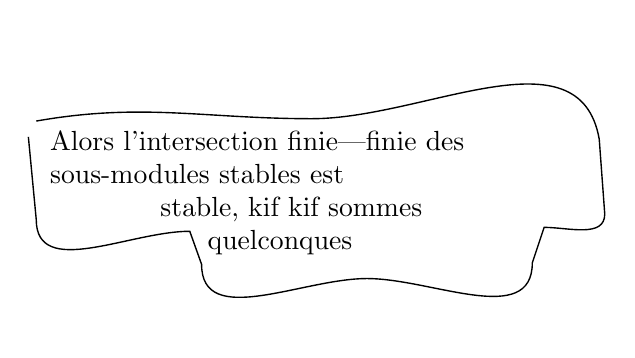
\begin{tikzpicture}[x=1cm,y=1cm]\node[anchor=north west,align=left,text width=7cm,inner sep=2pt](s) at (0,0){Alors l'intersection \unsure{\deleted{finie}|finie} des\\sous-modules stables est\\\hspace*{1.4cm}stable, kif kif sommes\\\hspace*{2cm}quelconques};\draw[line width=.5pt] (-.1,.05) to[out=10,in=180] (3.4,.08) to[out=0,in=100] (7.05,-.18)--(7.12,-1.13) to[out=-90,in=0] (6.35,-1.3)--(6.2,-1.75) to[out=-90,in=0] (4.1,-1.95) to[out=180,in=-90] (2,-1.77)--(1.85,-1.35) to[out=180,in=-90] (-.1,-1.2)--(-.2,-.15);\end{tikzpicture}}
% @ 23
b) $M/M''$ est \inserted{$\unsure{A|\wedge}$} plat

% @ 24
c) $M''$ facteur direct dans $M$.

% @ 24 left margin
% slanted
\margin{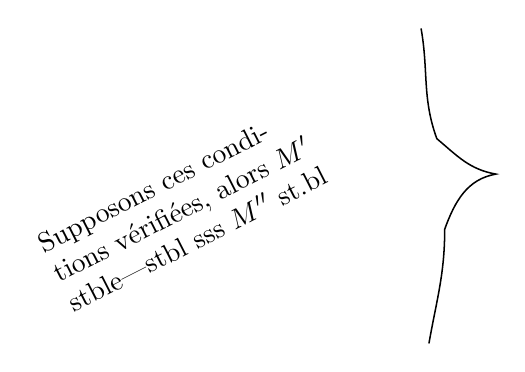
\begin{tikzpicture}[x=1cm,y=1cm]\node[rotate=27,align=left,text width=4.5cm,inner sep=2pt](s) at (0,0){\deleted{Supposons ces conditions vérifiées, alors $M'$ \unsure{stble|stbl} sss $M''$ st.bl}};\draw[line width=.55pt] (2.65,2.1) to[out=-80,in=110] (2.85,.7) to[out=-40,in=170] (3.6,.25) to[out=190,in=70] (2.95,-.45) to[out=-90,in=80] (2.75,-1.9);\end{tikzpicture}}
% @ 25
\deleted{ou $A$ \unsure{libre bien}.}

% @ 26–29
Dans le cas $A$ libre [plus gén. somme de modules proj. de t. f.] on voit que $M'$ est \unsure{st.bl|st.ble} sss $M'$ est \deleted{stable sous l'action de $\check{A}$.} un sous-$\check{A}$-module. On trouve donc

% @ 30–32
\uline{Proposition} Si $A$ est somme de modules proj. de t. f., alors un sous-$k$-module \deleted{de} $A$-comodule est st.bl sss il est \deleted{stable sous l'op.} \unsure{un|est} sous $\unsure{\check{A}|\tilde{A}}$-module.
% archive sheet number: 28
